\section{Development - 31/03/2019}
I have decided to pursue the 'Ethernet' approach, which is to use an \ac{SFP}
module, the same as all the other \ac{FSO} approaches do. The idea will be
to break out an \ac{SFP} module using a breakout board so that the laser
and photodiode can be attached. This should then be able to drive the system
much higher and provide a much faster link (gigabit).

The \ac{SFP} specification can be found here:
\url{http://www.kt.agh.edu.pl/~lason/SFP/TRX100007/SCP6Gx8c.pdf}

\paragraph{\textbf{Components ordered}}
\begin{itemize}
\item{3 x \ac{SFP} to SMA Adapter
(\url{https://shop.trenz-electronic.de/en/TE0422-02-SFP-2-SMA-Adapter?path=Trenz_Electronic/Accessories/SFP/TE0422/REV02})}
\item{4 x SMA cables
(\url{https://www.thorlabs.com/thorproduct.cfm?partnumber=CA2912})}
\item{2 x Gigabit ethernet media converters - for the power supplies mainly.
(\url{https://www.amazon.com/TP-Link-Ethernet-Converter-Supporting-MC220L/dp/B003CFATL0})}
\end{itemize}

\section{Development - 03/04/2019}
The aim is firstly to study how the signalling works for the \ac{SFP}
modules. These are already available inside the KORUZA modules. The modules
were taken from the control laboratory, from Ibrahima
(\href{mailto:ibrahima.ndoye@kaust.edu.sa}{ibrahima.ndoye@kaust.edu.sa}).

Two KORUZA systems have been dismantled and I have removed the following
components:

\paragraph{\textbf{KORUZA components removed}}
\begin{itemize}
\item{TP-Link MC220L}
\item{KORUZA \ac{SFP} breakout boards. See here for circuit diagrams:
\url{https://github.com/IRNAS/KORUZA/blob/master/electronics/KORUZA_SFPextension_plug/SFPextension.PDF}
and \url{https://github.com/IRNAS/KORUZA/blob/master/electronics/KORUZA_SFPextension_socket/SFPextensionSplit.PDF}}
\item{KORUZA \ac{SFP} module}
\end{itemize}

As well as this, I also have the following:

\paragraph{\textbf{Other components used}}
\begin{itemize}
\item{Power Supply (used to power TP-Link boxes). Set to 5V, 1.4A maximum
(as each TP-Link box can draw around 0.6A)}
\item{Optical Fibre (for testing)}
\item{\ac{SFP} to Ethernet module (for testing)}
\item{Raspberry Pi (for testing)}
\item{Router}
\item{2 x Ethernet cables (between TP-Link boxes and Raspberry Pi / Router)}
\item{Oscilloscope to check signals}
\end{itemize}

The Raspberry Pi is set up as an Ethernet bridge to Wifi as described here:
\url{https://www.raspberrypi.org/documentation/configuration/wireless/access-point.md}.
In particular the section "\textbf{Using the Raspberry Pi as an access
point to share an internet connection (bridge)}".

Note I also have to do the following after following the instructions
\begin{lstlisting}
	sudo systemctl unmask hostapd
	sudo systemctl enable hostapd
	sudo systemctl start hostapd
\end{lstlisting}

\section{Development - 07/04/2019}
Note that the Raspberry Pi WiFi does not seem to be stable. Was told by previous
student that it might require an external WiFi adapter in order to function
properly. Nevertheless we're going to throw it away anyway so doesn't matter.

At first I tried to point the \ac{SFP} modules at each other but the Link was
not stable. I then tried using an optical fibre but it would not plug in
properly. \textbf{Update 09/04/2019: this is indeed because the laser is
missing a part. It should have a plastic header on the front of it; I assume
this was removed (there looks to be burn marks on the front) for the
KORUZA system.}
Instead of this, I managed to get two \ac{SFP} to Ethernet modules
and plugged then into each TP-Link box. This was enough to allow the Link
to be set up.

If the infra-red \ac{SFP} modules are aligned properly, the link is stable.
I am seeing some packet loss though this may be because the link isn't aligned
as perfectly as it could be (it's just on the table with no proper optical
alignment).

Next steps are to measure the signals (TX / RX differential ones) that go over
the SATA connector to the external \ac{SFP} cage. From this we can then
determine that the \ac{SFP} module can be pretty basic and we can just attach
our laser / photodiode. We also need to check what is in the \ac{I2C} EEPROM
memory and copy it out so that we can 'pretend' to be the same module when
we use the breakout board.

I used the Raspberry Pi that comes with Koruza as it already has the breakout
to the I2C device. This is what is in the I2C EEPROM memory, using the
following command:

\begin{lstlisting}
	i2cdump 1 0x50 i

     0  1  2  3  4  5  6  7  8  9  a  b  c  d  e  f    0123456789abcdef
00: 03 04 00 00 00 00 08 00 00 00 00 01 0d 00 00 00    ??....?....??...
10: 00 00 64 00 43 49 53 43 4f 2d 41 56 41 47 4f 20    ..d.CISCO-AVAGO 
20: 20 20 20 20 01 00 17 6a 41 42 43 55 2d 35 37 31        ?.?jABCU-571
30: 30 52 5a 2d 43 53 32 20 20 20 20 20 41 0c c1 13    0RZ-CS2     A???
40: 00 10 00 00 41 47 4d 31 32 34 35 32 32 56 35 20    .?..AGM124522V5 
50: 20 20 20 20 30 38 31 31 31 30 20 20 00 00 00 ab        081110  ...?
60: 00 00 06 11 36 c9 64 cf 43 18 00 cc 0f 1e 82 f0    ..??6?d?C?.?????
70: 80 ec 6f 00 00 00 00 00 00 00 00 00 4a af 0d b2    ??o.........J???
80: ff ff ff ff ff ff ff ff ff ff ff ff ff ff ff ff    ................
90: ff ff ff ff ff ff ff ff ff ff ff ff ff ff ff ff    ................
a0: ff ff ff ff ff ff ff ff ff ff ff ff ff ff ff ff    ................
b0: ff ff ff ff ff ff ff ff ff ff ff ff ff ff ff ff    ................
c0: ff ff ff ff ff ff ff ff ff ff ff ff ff ff ff ff    ................
d0: ff ff ff ff ff ff ff ff ff ff ff ff ff ff ff ff    ................
e0: ff ff ff ff ff ff ff ff ff ff ff ff ff ff ff ff    ................
f0: ff ff ff ff ff ff ff ff ff ff ff ff ff ff ff ff    ................

	i2cdump 1 0x56 i

     0  1  2  3  4  5  6  7  8  9  a  b  c  d  e  f    0123456789abcdef
00: 01 40 01 6d 01 41 0c c1 0c 01 c0 01 00 0f 20 01    ?@?m?A??????.? ?
10: 4c ff 0e 00 78 00 00 00 00 00 00 00 00 00 f0 00    L.?.x.........?.
20: 01 40 01 6d 01 41 0c c1 0c 01 c0 01 00 0d 20 01    ?@?m?A??????.? ?
30: 4c ff 0e 00 78 00 00 00 00 00 00 00 00 00 f0 00    L.?.x.........?.
40: 01 40 01 6d 01 41 0c c1 0c 01 c0 01 00 0d 20 01    ?@?m?A??????.? ?
50: 4c ff 0e 00 78 00 00 00 00 00 00 00 00 00 f0 00    L.?.x.........?.
60: 01 40 01 6d 01 41 0c c1 0c 01 c0 01 00 0d 20 01    ?@?m?A??????.? ?
70: 4c ff 0e 00 78 00 00 00 00 00 00 00 00 00 f0 00    L.?.x.........?.
80: 01 40 01 6d 01 41 0c c1 0c 01 c0 01 00 0d 20 01    ?@?m?A??????.? ?
90: 4c ff 0e 00 78 00 00 00 00 00 00 00 00 00 f0 00    L.?.x.........?.
a0: 01 40 01 6d 01 41 0c c1 0c 01 c0 01 00 0d 20 01    ?@?m?A??????.? ?
b0: 4c ff 0e 00 78 00 00 00 00 00 00 00 00 00 f0 00    L.?.x.........?.
c0: 01 40 01 6d 01 41 0c c1 0c 01 c0 01 00 0d 20 01    ?@?m?A??????.? ?
d0: 4c ff 0e 00 78 00 00 00 00 00 00 00 00 00 f0 00    L.?.x.........?.
e0: 01 40 01 6d 01 41 0c c1 0c 01 c0 01 00 0d 20 01    ?@?m?A??????.? ?
f0: 4c ff 0e 00 78 00 00 00 00 00 00 00 00 00 f0 00    L.?.x.........?.
\end{lstlisting}

We need to replicate this. Note the EEPROM specification is from section 8.1
in \url{http://www.kt.agh.edu.pl/~lason/SFP/TRX100007/SCP6Gx8c.pdf}.

\section{Development - 08/04/2019}
I have managed to capture some sort of signal on the differential outputs
of the SATA connection which provides the signalling to the \ac{SFP} connector.
Unfortunately the signal isn't very clean so I'm trying to make that better.

This is a useful resource about the timings:
\url{https://electronics.stackexchange.com/questions/328412/how-gigabit-ethernet-is-achieved-in-fiber-optics}

\subsection{Finding out more information about differential to single ended
conversion}
I am trying to figure out how to take the differential signals that are ouput
from the SFP connection and make them into single ended signals.
They do it here: \url{https://osmocom.org/projects/misc-hardware/wiki/Sfp-experimenter}
Also here: \url{https://github.com/aewallin/SFP2SMA_2018.03}. Looks like this
one is faster. It uses Mini-Circuits ADT2-1T transformers (see \url{https://www.minicircuits.com/pdfs/ADT2-1T.pdf}).
Note we're only using a 125Mhz clock (as 1 Gbps using 8b/10b encoding).
Maybe we should get some of these? \url{https://www.analog.com/media/en/reference-design-documentation/reference-designs/5693022520349015544867851905SFP_RDK_pra.pdf}

\section{Development - 09/04/2019}

Something interesting here (with relation to the previous Analog Devices
reference design)
\url{https://www.arrow.com/en/reference-designs/laser-driver-for-gb-ethernet-switch/6ce61f01a20a56fa532aa09927c84d22}
Another one here (this is the 10G one): \url{http://www.ti.com/tool/TIDA-00088}
And more: \url{https://www.analog.com/en/products/landing-pages/001/sfp-chipset-and-reference-design.html}.
I contacted Analog Devices to ask if we can get the reference design from them.

Current system is using the following:
\begin{itemize}
\item{Thorlabs DET10A2 Si Biased Detector}
\item{Osram 1.6 Watt Blue Laser Diode in TO56 Package}
\end{itemize}

\subsection{\ac{AGC}}
We really need to think about \ac{AGC} and how it's supposed to function. It
seems that in typical \ac{SFP} connections they control both the TX side
by utilising a photodiode in the transmitter to adjust the power; in the RX
side the RX power is adjusted too, probably by measurements.
Looks like we may need some sort of microcontroller to adjust the \ac{AGC}; this
is how it's done in other systems.

\subsection{What's in the IRNAS SFP connector}
I took apart the IRNAS SFP connector. The main chip on it is this:
\url{https://www.datasheetarchive.com/pdf/download.php?id=7a1d8924e962602762f27f57b62de6accd74e5&type=P&term=M0201x}
The suggested single ended to differential converter is M0201x. Here's an
example
\url{https://www.datasheetarchive.com/pdf/download.php?id=1450622d93878decd445ca73f09843c5b2a176&type=P&term=M02011%252F13%252F00}

It looks like we need a laser driver for the TX (\url{https://www.laserdiodecontrol.com/laser-diode-driver-basics-and-fundamentals#what-is-a-laser-diode-driver-link},
another one \url{https://www.teamwavelength.com/laser-diode-driver-basics/})
and for the RX a "Transimpedance Amplifier with AGC".

Looks like the laser is a \ac{BOSA}. Here's a typical diagram of the pins:

\begin{figure}[H]
  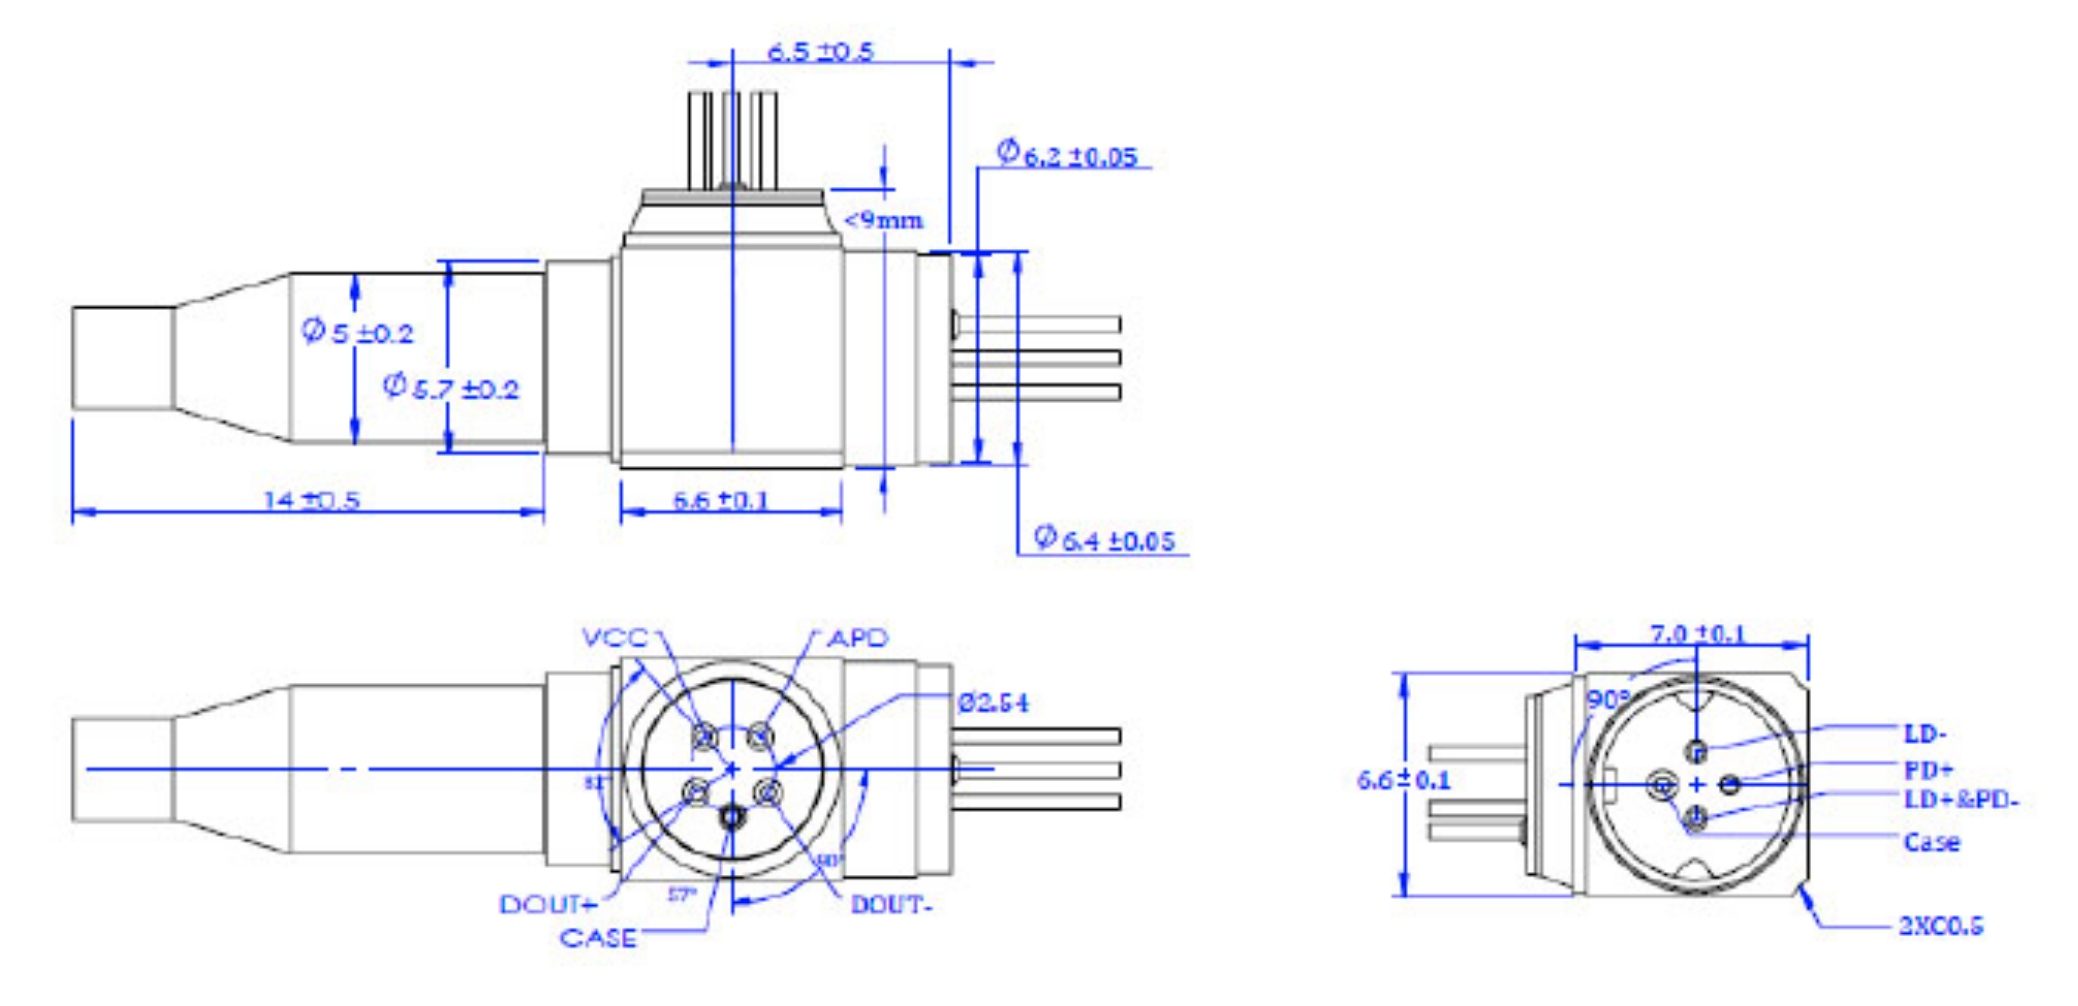
\includegraphics[width=0.8\textwidth]{bosa.png}
  \caption{Generic \ac{BOSA} pinout diagram}
  \label{fig:bosa}
\end{figure}

I wonder if we can get a \ac{BOSA} setup? Otherwise we'll need separate TOSA
and ROSA setups.
TOSA (want style A or B.. or C?!?) - \url{https://www.thorlabs.com/NewGroupPage9.cfm?ObjectGroup_ID=7}
L520P50 (520nm) - \url{www.thorlabs.com/_sd.cfm?fileName=QTN010002-S01.pdf&partNumber=L520P50}.

(Note we want to use either 450nm or 520nm lasers)
Current OSRAM laser does not provide a monitoring photodiode (not sure if
this is necessary).

\subsubsection{Heatsinks}
A quick note about heatsinks - the lasers need good ones! Otherwise they don't
transmit at the required frequency.

\section{Development - 10/04/2019}
Asked and received a specification for the KORUZA \ac{SFP} module that they
have (GSB-1235S-L4ID). See the specification in this folder.

Ok so we can use either \url{https://cdn.macom.com/datasheets/M02016.pdf} or
\url{https://cdn.macom.com/datasheets/M02015.pdf}, depending on which one
is the better part, as the Transimpedance Amplifier.

Here's a fun paper about using a transimpedance amplifier for visible light communication \cite{fuada_putra_aska_adiono_2016}

\subsection{Duplex}
Omar mentioned a good point - is a 1 gigabit SFP connection full duplex or half
duplex. The answer is that it's full duplex (they use different colour lights
for each end). So we'll need to ensure we either do the same, or we space our
lasers / receivers far enough apart that they won't interfere with each other.

Emailed KORUZA again to ask if they have a spec for the \ac{BOSA} module as it
definitely must have a pre-amplifier integrated into it, though I'm not sure
which one. Looking at the documentation it seems that they want the
pre-amplifier mounted as close to the receiver as possible.

\section{Development - 11/04/2019}
What we're looking for is a PIN-TIA (or similar e.g. APD-TIA) for the receiver.
This is a photodiode with an integrated trans-impedance amplifier.
E.g. \url{https://www.kyosemi.co.jp/en/communication/ingaas_pin-tia_receiver/kpdx1gk/}

However, these don't seem to be available for visible light - only for
infra-red.

Here's another interesting paper \url{https://www.researchgate.net/publication/313998403_Automatic_Gain_Control_Circuit_for_Mobility_Visible_Light_Communication_System_using_LM13700}

I completed some more of the training modules.



\section{Development - 14/04/2019}
Completed all training modules (including laser training).

Completed:
\begin{itemize}
\item{Lab Safety Training}
\item{Hazardous Waste Training}
\item{Particularly Hazardous Substance}
\item{Emergency Incident Preparedness Training}
\item{Laser Safety Training}
\end{itemize}

Asked to do more training modules.

Completed:
\begin{itemize}
\item{Hydrofluoric Acid Training}
\item{UV Safety Training}
\item{Fume Hood Safety Training}
\end{itemize}

\section{Development - 15/04/2019}
Completed training modules

\begin{itemize}
\item{Liquid Nitrogen Training}
\item{Compressed Gas Cylinder}
\end{itemize}

I stumbled across the RONJA \url{https://en.wikipedia.org/wiki/RONJA} page
which led me to \url{http://electric2.ee.psu.ac.th/~ton/FSO_Ronja_TENCON2006_Final2.pdf}.
This is interesting because they're not using a 'traditional' transimpedance
preamplifier design. What I don't really understand is why not, and is this
suitable for our application or is the bandwidth too small?

There's some more information here:
\url{https://en.wikipedia.org/wiki/Visible_light_communication}

The Wikipedia page on TIA is quite useful:
\url{https://en.wikipedia.org/wiki/Transimpedance_amplifier}
(On that note, why is the comparator there? Why not just plug the photodetector
into the negative side of the op-amp...)

I have sent this to Corelabs:

Hi,

I'm looking for some help / advice on integrating a photodiode with an existing laser driver / amplifier.

The setup is thus - I want to integrate a visible light laser and photodiode that detects visible light with an existing SFP module, which currently has an infra-red transmitter / receiver in a BOSA form attached to it.

The SFP module has this device on board:

\url{https://www.datasheetarchive.com/pdf/download.php?id=7a1d8924e962602762f27f57b62de6accd74e5&type=P&term=M0201x}

The visible light laser I think is quite simple to integrate (should be just a plug and play as long as I choose the right component).

The photodiode, however, requires a transimpedance amplifier, according to the diagram on the first page (labelled M0201x). I believe this is the right part:

\url{https://cdn.macom.com/datasheets/M02015.pdf}

As can be seen from section 4.3 (page 22) the amplifier is supposed to be soldered directly to the TO-Can. I believe something like this:

\url{http://www.rmtltd.ru/products/submounts/to46/}

The photodiode would normally be mounted inside the TO-Can package, however we'll need to attach it to the M02015. I was aiming to use a photodiode such as:

\url{www.thorlabs.com/_sd.cfm?fileName=0637-S01.pdf&partNumber=FDS100}

and then soldering the output pins to the input PINK and PINA pins.

Do you think this will work? I'm mostly concerned about not having the photodiode and transimpedance amplifier attached to the same part. I'm also unsure if I have selected the right combination of photodiode / transimpedance amplifier, as I'm struggling to understand whether they will interface correctly (ie. the voltages are the same etc).

I'd really appreciate any advice and whether you think this is possible / the right approach.

I have attached photos of the SFP module with the BOSA part in the foreground (this is the part I want to change).

Many thanks,
Chris Bainbridge

\section{Development - 16/04/2019}
Ambient light sensors - what are these? Can we get one that will do what we
want? Something like \url{http://www.ti.com/product/OPT301}

OK so they do something like what I'm trying to do here:
\url{https://www.osapublishing.org/DirectPDFAccess/804494B1-E820-A80B-F9AF4E743C98EDE5_303458/oe-22-22-27203.pdf?da=1&id=303458&seq=0&mobile=no}

In particular the following extraction:

An optical short-pass filter with a cutoff wavelength of 500 nm and an optical
convex lens (5 cm focal length) was mounted in front of the PIN photodiode
(HAMAMATSU  S10784). An trans-impedance amplifier (TIA) MAX3665 (8KOhm
gain, 470MHz bandwidth) was used to amplify electrical current signal
of photodiode (PD), then a differential amplifier (ADA4937-1) circuit
with post-equalization boosted the signal level up to the operation range of
the error bit-error-ratio (BER) tester (Agilent  81250). The receiver also
consists a wideband limiting amplifier (MAX3768) with a gain of 55 dB,
which could provide low voltage positive emitter-coupled logic (LVPECL) output
interface.

HOW is the TIA integrated though?!?

OK, looks like we could use a surface mount PIN photodiode. E.g.
\url{https://www.vishay.com/docs/81643/temd5080.pdf}

\section{Development - 17/04/2019}
Popped down to the Electronics lab (in the Core Labs area). Had a chat with
them about mounting a transimpedance amplifier. They said that wire bonding
is something they can do (with help from the nanofabrication people), which
means we can mount the amplifier.
They say they can do normal, reflow and wire bonding so we should be good to
order some parts (just need to check dimensions etc).

Photoreceiver. This is possibly what we want. I've sent some emails to quite
a lot of companies - we'll see what they come back with!

Ooh ooh I think I've found what we want:
\url{http://osioptoelectronics.com/standard-products/silicon-photodiodes/photodiode-amplifier-hybrids/1-25gbps-photodiode-amplifier-hybrids.aspx}

\section{Development - 18/04/2019}
Spent the morning in a meeting with the Control Group. Some interesting things
to take away from that:

\begin{itemize}
\item{Not sure whether the camera can actually detect the laser beam. It was
suggested that instead, we use the camera to track the laser beam that is
directed onto the surface near the photodiode. The photodiode and camera would
be attached to the same motor, so that when the camera moves the photodiode
also moves and thus compensate.}
\item{What is the maximum distance the camera can work at?}
\item{What is the minimum movement that the motors can do? Is this minimal
enough for the precision we need?}
\item{How accurate is the tracking?}
\end{itemize}

Sent some more emails this afternoon asking for more information on the
OSI Optoelectronics product, and also asking for some to be delivered.

Another one:
\url{https://www.finisar.com/sites/default/files/downloads/hfd7180-001_8_gbps_850nm_pin-preamp_lc_rosa_package_product_specification_revb00_022015.pdf}

\section{Development - 21/04/2019}
Thought I'd do some research on control systems. Haven't seen that anyone
has actually done anything on it (I believe 'why don't we just use a camera'
was the extent of the research).

Here's a good summary:
\url{https://web.njit.edu/~rojasces/publications/2018kayrocomst.pdf}

\section{Development - 22/04/2019}
Found this:
\url{https://pdfserv.maximintegrated.com/en/an/AN2360.pdf}
This describes that Honeywell make the ROSA part. Have emailed them to ask if
we can get a part made or whether they have something available.

Nope Honeywell VCSEL doesn't exist anymore. Finisar bought them and then Finisar
was bought by II-VI. Have emailed them.

It seems to be almost impossible to get hold of a small number of M02016 parts.
You need to buy at least 2000 of them. What the hell.

\section{Development - 24/04/2019}
Have had an email conversation with some guys from OSI Optoelectronics.
Am awaiting a response but he said that their product should work with the
light ranges we're targeting, so it should hopefully just be a matter of getting
hold of them. This is in reference to this
\url{http://www.osioptoelectronics.com/standard-products/silicon-photodiodes/photodiode-amplifier-hybrids/1-25gbps-photodiode-amplifier-hybrids.aspx}

Also had another email conversation with Hammatsu, who say they don't have
anything but can possibly build something depending on (basically) whether there
is any point and whether it is good for them from a business point of view.
Am awaiting a response.

Started to look into the control mechanisms and whether a camera is good
enough. I don't believe it is. Lots of the literature seems to refer to
utilising maneouverable lenses or mirrors. See
\url{http://www.sbsstc.ac.in/icccs2014/Papers/Paper50.pdf}
\url{https://www.osapublishing.org/oe/fulltext.cfm?uri=oe-25-15-17971&id=369981}
\url{https://www.researchgate.net/publication/233854960_Smart_Transmitters_and_Receivers_for_Underwater_Free-Space_Optical_Communication}
Have sent emails to the control guys asking why they think a camera will
work.

I have a meeting with TK tomorrow wahey!

Had a look at diversity in radios. Here's some fun links:
\url{https://en.wikipedia.org/wiki/Diversity_combining}
\url{https://site.uottawa.ca/~sloyka/elg4179/Lec_11_ELG4179.pdf}

